\documentclass{article}
\usepackage{graphicx} % Required for inserting images
\usepackage{algorithm}
\usepackage{algpseudocode}
\usepackage{amssymb} 
\usepackage{amsmath}
\usepackage{hyperref}
\usepackage{float}
\usepackage[utf8]{inputenc}
\usepackage{listings}
\usepackage{xcolor}
% disable all line numbers in algpseudocode
\algrenewcommand\alglinenumber[1]{}

% Configure the appearance of Python code
\lstset{
  language=Python,
  basicstyle=\ttfamily\small,
  keywordstyle=\bfseries\color{blue},
  commentstyle=\itshape\color{gray},
  stringstyle=\color{teal},
  showstringspaces=false,
  frame=single,               % draw a box around the code
  numbers=left,               % show line numbers on the left
  numberstyle=\tiny\color{gray},
  stepnumber=1,               % number every line
  numbersep=8pt,
  breaklines=true,
  postbreak=\mbox{\textcolor{red}{$\hookrightarrow$}\space}
}


\title{CS238 Homework 1}
\author{Fatima Nawmi}
\date{April 2025}

\begin{document}

\maketitle

\section{Question 1}

The outputs from the given test cases are as follows:
\begin{enumerate}
    \item Test case: {2(1), 3(1), 4(1), 5(1), 6(1), 7(2), 8(2), 10(1)}\\
No solution\\
    \item Test case: {1(9), 2(8), 3(7), 4(6), 5(5), 6(4), 7(3), 8(2), 9(1)}\\
The number of distinct solution(s): 1\\
Distinct solution: [0, 1, 2, 3, 4, 5, 6, 7, 8, 9]\\

    \item Test case: {1(1), 2(1), 3(2), 4(1), 5(2), 6(1), 7(1), 9(2), 10(1), 12(1), 14(1), 15(1)}\\
    The number of distinct solution(s): 1\\
    Distinct solution: [0, 5, 9, 12, 14, 15]\\
    \item Test case: {1(16), 2(15), 3(14), 4(13), 5(12), 6(11), 7(10), 8(9), 9(8), 10(9), 11(8), 12(7), 13(6), 14(5), 15(4), 16(3), 17(2), 18(1)}\\
    The number of distinct solution(s): 1\\
    Distinct solution: [0, 1, 2, 3, 4, 5, 6, 7, 8, 10, 11, 12, 13, 14, 15, 16, 17, 18]\\
\end{enumerate}

Code: \href{https://github.com/fatimanawmi/CS238/blob/main/PDP.py}{github}

\section*{Partial Digest Problem (Python)}

\begin{lstlisting}
# Partial Digest Problem
all_X = []

def checkSymmetry(sol1, sol2, width):
    temp = []
    for i in range(len(sol1)):
        temp.append(abs(sol1[i] - width))
    temp.sort()
    if len(temp) != len(sol2):
        return False
    for i in range(len(sol1)):
        if temp[i] != sol2[i]:
            return False
    return True

def inputFormat(data):
    L = list()
    data = data[1:-1]
    token = data.split(',')
    for i in range(len(token)):
        subToken = token[i].split('(')
        num = int(subToken[0])
        multicity = subToken[1].split(')')[0]
        for j in range(int(multicity)):
            L.append(num)
    return L

def Delete(y, L):
    for i in range(len(y)):
        L.remove(y[i])
    return L

def Add(y, L):
    for i in range(len(y)):
        L.append(y[i])
    return L

def multiset(X):
    deltaX = []
    for i in range(len(X)):
        for j in range(i + 1, len(X)):
            deltaX.append(abs(X[i] - X[j]))
    return deltaX

def multisetDiffInL(y, X, L):
    diff = []
    for i in range(len(X)):
        diff.append(abs(X[i] - y))
    for i in range(len(diff)):
        if diff[i] not in L:
            return False, diff
    return True, diff

def Place(L, X, width):
    if len(L) == 0:
        check = True
        X.sort()
        for sol in all_X:
            if checkSymmetry(X, sol, width):
                check = False
                break
        if check:
            all_X.append(X.copy())
        return
    y = max(L)
    flag, diff = multisetDiffInL(y, X, L)
    if flag:
        L = Delete(diff, L)
        X.append(y)
        Place(L, X, width)
        L = Add(diff, L)
        X.remove(y)
    flag, diff = multisetDiffInL(width-y, X, L)
    if flag:
        L = Delete(diff, L)
        X.append(width-y)
        Place(L, X, width)
        L = Add(diff, L)
        X.remove(width-y)
    return 

def PartialDigest(L):
    width = max(L)
    L.remove(width)
    X = [0, width]
    Place(L, X, width)

with open('input.txt', 'r') as file:
    lines = file.readlines()
    for line in lines:
        L = inputFormat(line.strip())
        PartialDigest(L)
        print("Test case:", line.strip())
        if len(all_X) == 0:
            print("No solution")
        else:
            print("The number of distinct solution(s):", len(all_X))
            print("Three distinct solution(s):", all_X[:3])
        all_X.clear()
\end{lstlisting}


\section{Question 2}


\begin{algorithm}[H]
\caption{Brute‑Force DDP}
\label{alg:ddp_bruteforce}
\begin{algorithmic}
  \State \textbf{Input:}
    \begin{tabular}[t]{@{}l@{}}
      $d_A,d_B$: multisets of fragment lengths from single digests A and B;\\
      $d_X$: multiset of fragment lengths from the double digest A+B.
    \end{tabular}
  \State \textbf{Output:} $(X_A,X_B)$, the sets of cut‐positions for A and B, or “no solution.”

  \Procedure{DoubleDigestBruteForce}{$d_A,d_B,d_X$}
    \State \textbf{let} $\mathit{totalLen}\gets$ sum of $d_A$
    \State \textbf{assert} sum of $d_B$ equals $\mathit{totalLen}$
    \ForAll{each ordering of fragments in $d_A$}
      \State compute $X_A$ as cumulative cut‐positions from that ordering
      \ForAll{each ordering of fragments in $d_B$}
        \State compute $X_B$ as cumulative cut‐positions from that ordering
        \State collect all fragment lengths induced by cuts in $X_A\cup X_B$
        \If{that multiset of lengths equals $d_X$}
          \State \Return $(X_A,X_B)$
        \EndIf
      \EndFor
    \EndFor
    \State \Return “no solution”
  \EndProcedure
\end{algorithmic}
\end{algorithm}

\subsection*{Performance Analysis: Brute‑Force for DDP}
Let $n$ be the number of fragments in the A-only digest ($|d_A|$), $m$ the number in the B-only digest ($|d_B|$), and $W$ the total DNA length ($W = \sum d_A = \sum d_B$). The algorithm maintains two cut sets $X_A$ and $X_B$, each storing enzyme cut positions (including 0 and $W$), with total size up to $n + m + 2$.\\
\textbf{Time Complexity:}
\begin{itemize}
  \item All permutations of $d_A$: $n!$
  \item All permutations of $d_B$: $m!$
  \item For each pair of permutations, compute $X_A$, $X_B$, merge cut sets, and generate fragments:
  \[
  O(n + m + W)
  \]
  \item \textbf{Total time:} 
  \[
  O(n! \cdot m! \cdot (n + m + W))
  \]
\end{itemize}

\textbf{Space Complexity:}
\begin{itemize}
  \item Temporary storage for cuts and fragment lists: $O(W)$
  \item No recursion stack; purely iterative
  \item \textbf{Overall space:} $O(W)$
\end{itemize}




\begin{algorithm}[H]
\caption{Branch‐and‐Bound approach for DDP}
\label{alg:place}
\begin{algorithmic}
 \State \textbf{Input:}
    \begin{tabular}[t]{@{}l@{}}
      $d_A,d_B$: multisets of fragment lengths from single digests A and B;\\
      $d_X$: multiset of fragment lengths from the double digest A+B.
    \end{tabular}
  \State \textbf{Output:} $(X_A,X_B)$, the sets of cut‐positions for A and B, or “no solution.”
  \Procedure{Place}{$d_A, d_B, d_X, X,\,\mathit{nextSide}$}
    \If{$d_A = \varnothing $ and $d_B = \varnothing$}
      \State \Return $(X[A],\,X[B])$
    \EndIf

    \Comment{Pick which enzyme to use this round}
    \If{$\mathit{nextSide} = \texttt{A}$ \textbf{and} $d_A \neq \varnothing$}
      \State $ \mathit{side} \gets \texttt{A}$
    \ElsIf{$\mathit{nextSide} = \texttt{B}$ \textbf{and} $d_B \neq \varnothing$}
      \State $ \mathit{side} \gets \texttt{B}$
    \ElsIf{$d_A \neq \varnothing$}
      \State $ \mathit{side} \gets \texttt{A}$
    \Else
      \State $ \mathit{side} \gets \texttt{B}$
    \EndIf

    \Comment{Loop over the chosen side’s fragments}
    \ForAll{$y \in d_{\mathit{side}}$}
      \State $Y \gets X[A] \cup X[B] \cup \{y\}$
      \State let $Y' \gets \mathrm{sort}(Y)$

      \Comment{Build the partial double‐digest fragments so far}
      \State $d_{X'} \gets []$
      \For{$i = 2$ \textbf{to} $|Y'|$}
        \State append $(Y'_i - Y'_{\,i-1})$ to $d_{X'}$
      \EndFor

      \If{$\mathrm{multiset}(d_{X'}) \subseteq \mathrm{multiset}(d_X)$}
        \Comment{Accept $y$, recurse, then backtrack}
        \State remove one copy of $y$ from $d_{\mathit{side}}$
        \State $X[\mathit{side}] \gets X[\mathit{side}] \cup \{y\}$
        \State \Call{Place}{$d_A, d_B, d_X, X,\,\mathrm{opposite}(\mathit{side})$}
        \State $X[\mathit{side}] \gets X[\mathit{side}] \setminus \{y\}$
        \State re‑insert $y$ into $d_{\mathit{side}}$
      \EndIf
    \EndFor

    \State \Return \textsf{"no solution"}
  \EndProcedure
\end{algorithmic}
\end{algorithm}

\subsection*{Performance Analysis: Branch-and-Bound for DDP}



\subsubsection*{Time Complexity}

\begin{itemize}
  \item \text{Recursion depth:} Up to $n + m$, since one cut is placed per level.
  \item \text{Branching factor:} Up to $\max(n, m)$ choices at each level.
  \item \text{Cost per node:}
    \begin{itemize}
      \item Merging and sorting cut positions: $O((n + m) \log(n + m))$
      \item Computing fragment lengths and subset check: $O(n + m)$
    \end{itemize}
  \item \text{Worst-case total runtime:}
    \[
      T(n, m) = O((n + m)! \cdot (n + m) \log(n + m))
    \]
\end{itemize}

\subsubsection*{Space Complexity}

\begin{itemize}
  \item \text{Recursion stack:} Depth at most $n + m$
  \item \text{Cut set storage:} Up to $n + m + 2$ per frame
  \item \text{Auxiliary data (e.g., multisets):} $O(n + m)$
  \item \text{Overall space:}
    \[
      \text{Worst-case: } O((n + m)^2), \quad \text{Optimized (in-place): } O(n + m)
    \]
\end{itemize}

\section{Question 3}

Code for an implementation that counts the number of occurrences of each l-mer in a
string of length n: \href{https://github.com/fatimanawmi/CS238/blob/main/lmer.py}{github}

Complete Bacterial Genome: \href{https://www.ebi.ac.uk/ena/browser/view/CP011331}{Escherichia coli O104:H4 str. C227-11, complete genome.
}



\section*{L-mer Counting and Distribution Plot (Python)}

\begin{lstlisting}
import random
from collections import Counter
import matplotlib.pyplot as plt
import pandas as pd

# Function to count l-mers in a sequence
def count_lmers(seq, l):
    return Counter(seq[i:i+l] for i in range(len(seq)-l+1))

# Function to load a genome from a FASTA file
def load_fasta(path):
    seq = []
    with open(path) as f:
        for line in f:
            if line.startswith('>'):
                continue
            seq.append(line.strip().upper())
    return ''.join(seq)

# Parameters
l = 5
genome_path = 'CP011331.1.fasta'

# Load genome and count l-mers
genome_seq = load_fasta(genome_path)
genome_counts = count_lmers(genome_seq, l)
genome_dist = Counter(genome_counts.values())

# Generate a random sequence of the same length and count l-mers
random_seq = ''.join(random.choice('ACGT') for _ in range(len(genome_seq)))
random_counts = count_lmers(random_seq, l)
random_dist = Counter(random_counts.values())

# Prepare DataFrames for display
df_genome = pd.DataFrame(sorted(genome_dist.items()), columns=['Occurrences', 'Num_lmers'])
df_random = pd.DataFrame(sorted(random_dist.items()), columns=['Occurrences', 'Num_lmers'])

# Plot two distributions of l-mers using subplots
plt.figure(figsize=(12, 6))
plt.subplot(1, 2, 1)
plt.scatter(df_genome['Occurrences'], df_genome['Num_lmers'], color='blue', alpha=0.7, label='Genome')
plt.title(f'L-mers Distribution in Genome (l={l})')
plt.xlabel(f'Frequency of {l}-mers')
plt.ylabel(f'Number of distinct {l}-mers')
plt.legend()
plt.grid(True)


plt.subplot(1, 2, 2)
plt.scatter(df_random['Occurrences'], df_random['Num_lmers'], color='orange', alpha=0.7, label='Random')
plt.title(f'L-mers Distribution in Random Sequence (l={l})')
plt.xlabel(f'Frequency of {l}-mers')
plt.ylabel(f'Number of distinct {l}-mers')
plt.legend()
plt.grid(True)
plt.tight_layout()
plt.savefig('lmer_distribution_both.png')
plt.show()

# plot a combined plot for genome and random sequence
plt.figure(figsize=(10, 6))
plt.scatter(df_genome['Occurrences'], df_genome['Num_lmers'], color='blue', label='Genome')
plt.scatter(df_random['Occurrences'], df_random['Num_lmers'], color='red', label='Random')
plt.title(f'L-mers Distribution (l={l})')
plt.xlabel(f'Frequency of {l}-mers')
plt.ylabel(f'Number of distinct {l}-mers')
plt.legend()
plt.grid(True)
plt.tight_layout()
plt.savefig('lmer_distribution.png')
plt.show()
\end{lstlisting}

\begin{figure}[H]
    \centering
    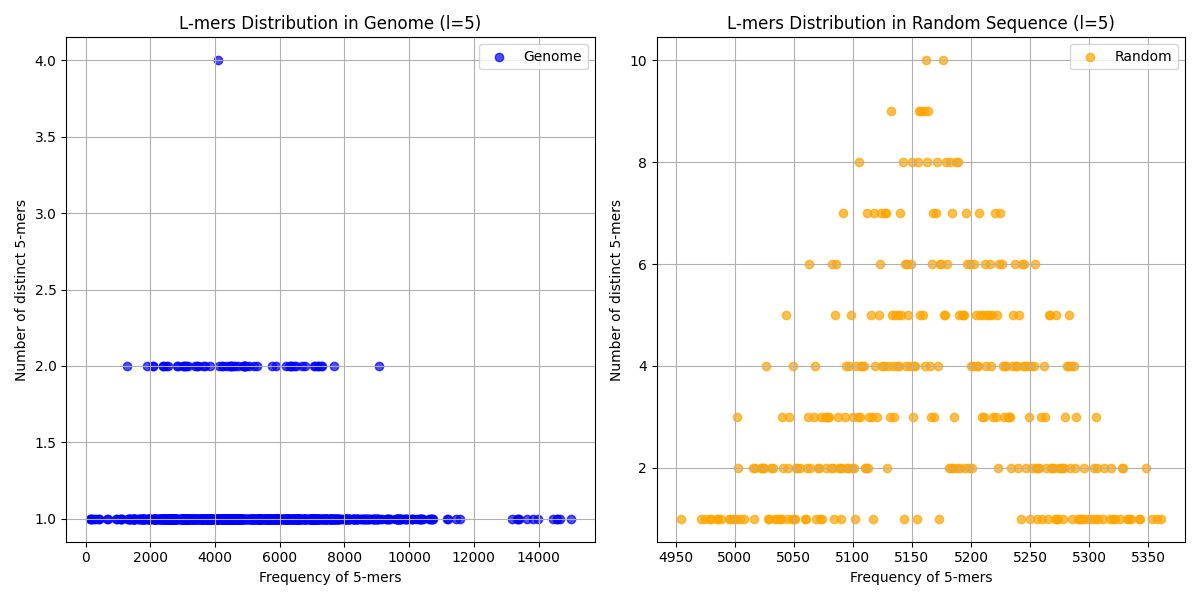
\includegraphics[width = \linewidth]{lmer_distribution_both.png}
     \caption{L-mers Distribution (l={5})}
\end{figure}

\begin{figure}[H]
    \centering
    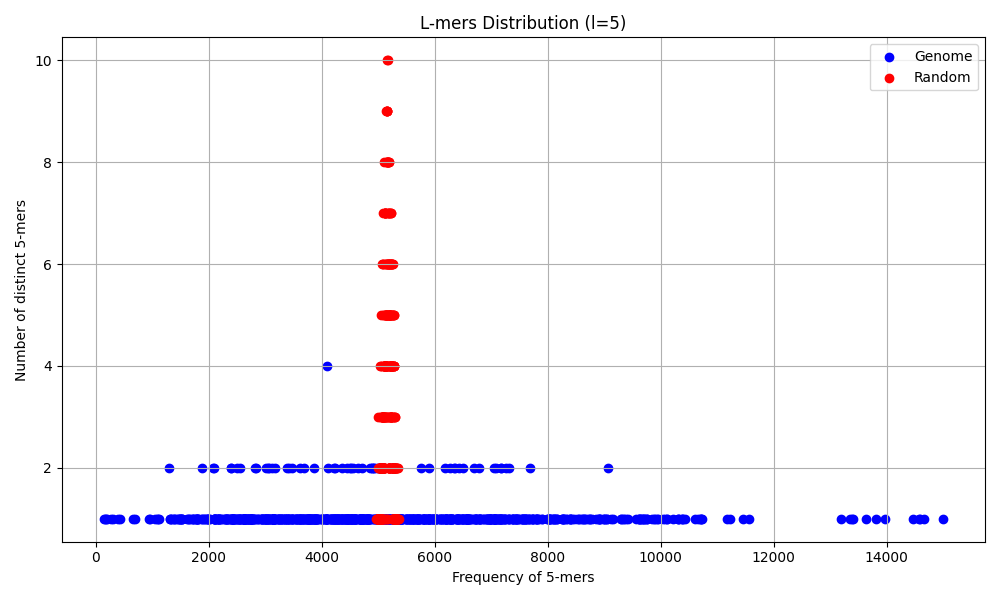
\includegraphics[width = \linewidth]{lmer_distribution.png}
     \caption{L-mers Distribution (l={5}) Combined}
\end{figure}

\subsection*{Observation}
The bacterial genome’s 5-mer frequency profile is much more dispersed and skewed compared to a random sequence of the same length. In the random control almost every 5-mer clusters closely around the mean count of approximately 5,000 occurrences, reflecting the narrow, Poisson like distribution expected when each base is chosen independently. In contrast the real genome exhibits a heavy tail of highly overrepresented motifs, with some appearing tens of thousands of times, while many 5-mers are rare or entirely absent. This overdispersion underscores the influence of biological features such as repeats, GC content biases, regulatory motifs and coding constraints, which drive k mer usage far from the uniformity of random DNA.


\section{Question 4}

\paragraph{Randomized k‑Means}
The \emph{randomized k‑Means} algorithm replaces the deterministic “assign to nearest centroid” step with a stochastic draw: each point \(x_i\) computes squared distances 
\[
d_j \;=\;\|x_i - \mu_j\|^2,
\]
forms a Gibbs distribution
\[
p_j \;=\;\frac{\exp(-d_j/T)}{\sum_{\ell=1}^k \exp(-d_\ell/T)},
\]
and samples its cluster according to \(\{p_j\}\). After all points are assigned, centroids are updated as the mean of their members, and the temperature is cooled via \(T\leftarrow\alpha T\). At high \(T\) the method explores broadly, while as \(T\to0\) it recovers Lloyd’s hard assignments; this annealed randomness helps escape poor local minima and yields more robust clustering.


\begin{algorithm}[ht]
\caption{Randomized $k$‑Means Clustering}
\label{alg:rand-kmeans}
\begin{algorithmic}[1]
\Require $X = \{x_1,\dots,x_n\}\subset\mathbb R^d$, \quad
         $k\in\mathbb N$, \quad
         $T_0>0$, \quad
         $\alpha\in(0,1)$, \quad
         $T_{\min}>0$
\State \textbf{Initialize:} 
\Statex \quad Choose centroids $\{\mu_j\}_{j=1}^k$ uniformly at random from $X$
\Statex \quad Set $T \gets T_0$
\While{$T > T_{\min}$ \textbf{and} not converged}
  \State \textbf{(1) Randomized assignment}
  \For{$i = 1,\dots,n$}
    \For{$j = 1,\dots,k$}
      \State $d_j \gets \|x_i - \mu_j\|^2$
      \State $w_j \gets \exp\bigl(-\,d_j / T\bigr)$
    \EndFor
    \State $p_j \gets \dfrac{w_j}{\sum_{\ell=1}^k w_\ell}
      \quad(\forall j)$
    \State Sample cluster index $s_i\in\{1,\dots,k\}$ with $\Pr(s_i=j)=p_j$
  \EndFor

  \State \textbf{(2) Centroid update}
  \For{$j = 1,\dots,k$}
    \State $\displaystyle
      \mu_j \;\gets\;
      \frac{1}{\bigl|\{i:s_i=j\}\bigr|}\sum_{i: s_i=j} x_i$
  \EndFor

  \State \textbf{(3) Cool down}
  \State $T \gets \alpha\,T$
\EndWhile
\State \Return $\{s_i\}_{i=1}^n,\;\{\mu_j\}_{j=1}^k$
\end{algorithmic}
\end{algorithm}

\subsection*{Performance Analysis}

\textbf{Time Complexity}\\
\begin{tabular}{@{}ll}
Iteration count: & Up to 
$\displaystyle I \;=\;\left\lceil\frac{\ln(T_{\min}/T_0)}{\ln(\alpha)}\right\rceil$ \\[6pt]
Branching factor: & Each of the $n$ points chooses among $k$ clusters \\[6pt]
Per‐iteration cost: & $O(n \times k \times d)$  
  \quad(distance computation $O(d)$ + sampling $O(k)$ per point)\\[6pt]
Worst‐case total runtime: & $O\bigl(I \times n\,k\,d\bigr)
  = O\bigl(n\,k\,d\;\ln(T_0/T_{\min})\bigr)$
\end{tabular}

\vspace{8pt}
\textbf{Space Complexity}\\
\begin{tabular}{@{}ll}
Stack depth: & $O(1)$ \quad(iterative algorithm)\\[6pt]
Centroid storage: & $O(k\,d)$ \\[6pt]
Auxiliary storage: & 
  \begin{tabular}[t]{@{}l@{}}
    — cluster labels: $O(n)$\\
    — weight vector for sampling: $O(k)$
  \end{tabular}\\[6pt]
Overall space: & $O(n + k\,d)$
\end{tabular}


\section{Question 5}


One simple way to get “bigger moves” out of Gibbs sampling is to switch from a single‐sequence update to a \emph{blocked Gibbs sampler} that re‐samples a whole subset of the starting positions at once.  Concretely, fix a block size \(b\) (e.g.\ \(b=2,3,\dots,t\)) and at each iteration:

\begin{enumerate}
  \item \textbf{Choose a random block.}  
    Pick a subset \(B\subseteq\{1,\dots,t\}\) of size \(\lvert B\rvert = b\).
  \item \textbf{Build profile on the complement.}  
    Remove the \(b\) \(\ell\)‑mers at positions \(\{s_i : i\in B\}\), and form the profile \(P\) from the remaining \(t-b\) sequences.
  \item \textbf{Re‑sample each block member.}  
    For each \(i\in B\), compute for every candidate position \(j\) in sequence \(i\) the Gibbs weight
    \[
      w^{(i)}_j \;=\;\Pr\bigl(\text{$\ell$‑mer at }j \mid P\bigr),
    \]
    normalize to obtain
    \[
      p^{(i)}_j \;=\;\frac{w^{(i)}_j}{\sum_{j'} w^{(i)}_{j'}},
    \]
    and then draw a new
    \[
      s_i \;\sim\;\mathrm{Categorical}\bigl(p^{(i)}_1,\dots,p^{(i)}_{n-\ell+1}\bigr).
    \]
  \item \textbf{Repeat} until convergence.
\end{enumerate}

\subsubsection*{Advantages}
\begin{itemize}
  \item  By re‑sampling multiple sequences in one shot, the sampler can more rapidly jump between very different alignments, especially when the true motif spans many sequences.
  \item  Large coordinated moves help the chain escape plateaus that single‐coordinate Gibbs might circle around.
\end{itemize}

\subsubsection*{Disadvantages}
\begin{itemize}
  \item Computing and sampling for \(b\) sequences costs \(O(b\,(n-\ell+1))\) rather than \(O(n-\ell+1)\).
  \item  Big moves can toss out partial good structure, so it may need more iterations (or a schedule that adapts \(b\)) to settle.
  \item  If blocks overlap improperly, we must adjust conditional distributions; for non‐overlapping blocks it remains a valid Gibbs sampler.
\end{itemize}

At the two extremes, \(b=1\) recovers the standard (slow‐moving) Gibbs sampler, while \(b=t\) becomes a fully parallel sampler that re‐assigns every sequence each round, which results in very fast jumping, but quite noisy.  Tuning \(b\) trades off exploration speed against stability.

\begin{algorithm}[ht]
\caption{Blocked Gibbs Motif Search}
\label{alg:blocked-gibbs-wordy}
\begin{algorithmic}[1]
\Require A collection of $t$ DNA sequences, each of length $n$
\Require Motif length $l$
\Require Block size $b$ (an integer between $1$ and $t$)
\Statex
\Comment \emph{Initialization}
\State Create an array \texttt{startPositions[1\,..\,t]}
\For{each sequence index $i$ from $1$ to $t$}
  \State Pick a random integer between $1$ and $n - l + 1$
  \State Set \texttt{startPositions[i]} to this integer
\EndFor
\State Let \texttt{bestPositions} $\gets$ \texttt{startPositions}
\State Let \texttt{bestScore} $\gets$ \texttt{Score}(\texttt{bestPositions})
\Statex
\Comment \emph{Main loop: continue until convergence}
\While{not converged}
  \State Randomly pick $b$ distinct sequence indices; call them \texttt{block}
  \State Let \texttt{complement} be all indices from $1$ to $t$ not in \texttt{block}
  \State Build a profile \texttt{P} from the subsequences of each sequence in \texttt{complement}, using their current start positions
  \For{each sequence index $i$ in \texttt{block}}
    \State Initialize an empty list \texttt{weights}
    \For{each candidate start position $j$ from $1$ to $n - l + 1$}
      \State Compute the probability that the length‑$l$ substring at position $j$ of sequence $i$ was generated by profile \texttt{P}
      \State Append this probability to \texttt{weights}
    \EndFor
    \State Normalize \texttt{weights} so they sum to 1
    \State Draw a random index from \texttt{weights} (i.e.\ sample according to their values)
    \State Update \texttt{startPositions[i]} to the sampled index
  \EndFor
  \State Let \texttt{currentScore} $\gets$ \texttt{Score}(\texttt{startPositions})
  \If{\texttt{currentScore} $>$ \texttt{bestScore}}
    \State \texttt{bestScore} $\gets$ \texttt{currentScore}
    \State \texttt{bestPositions} $\gets$ \texttt{startPositions}
  \EndIf
\EndWhile
\State \Return \texttt{bestPositions}, \texttt{bestScore}
\end{algorithmic}
\end{algorithm}

\subsection*{Performance Analysis}

\begin{itemize}
  \item \textbf{Time per iteration:}
    Building the profile costs $O\bigl((t-b)\,l\bigr)$;
    sampling $b$ sequences costs
    $O\bigl(b\,(n-l+1)\,l\bigr)\approx O(b\,n\,l)$.
    Thus the dominant term is $O(b\,n\,l)$.
  \item \textbf{Space:}
    Profiles store $\Sigma$ probabilities for each of the $l$ positions, hence the space requirement is
 $O\bigl(l\,\Sigma\bigr)$;
    weights array $O(n)$;
    start‐positions array $O(t)$.
\end{itemize}













\end{document}
